%
% Template for OPTCON course projects
%
\documentclass[a4paper,11pt,oneside]{book}
\usepackage[latin1]{inputenc}
\usepackage[english]{babel}
\usepackage{amsfonts}
\usepackage{amsmath}
\usepackage{amssymb,amsmath,color}
\usepackage{cite}
\usepackage{graphicx}
\usepackage{float}

\begin{document}
\pagestyle{myheadings}

%%%%%%%%%%% Cover %%%%%%%%%%%
\thispagestyle{empty}                                                 
\begin{center}                                                            
    \vspace{5mm}
    {\LARGE UNIVERSIT\`A DI BOLOGNA} \\                       
      \vspace{5mm}
\end{center}
\begin{center}
  
\includegraphics[scale=.27]{figs/logo_unibo}
\end{center}
\begin{center}
      \vspace{5mm}
      {\LARGE School of Engineering} \\
        \vspace{3mm}
      {\Large Master Degree in Automation Engineering} \\
      \vspace{20mm}
      {\LARGE Optimal Control} \\
      \vspace{5mm}{\Large\textbf{Optimal Control of a Quadrotor with Suspended Load}}                  
      \vspace{15mm}
\end{center}
\begin{flushleft}                                                                              
     {\large Professor: \textbf{\@ Giuseppe Notarstefano}} \\        
      \vspace{13mm}
\end{flushleft}
\begin{flushright}
      {\large Students:GUTU ABEYA TEFERA
                        \\DEBADIPTA JHA
                        \\ZERUN HUI}\\
\end{flushright}        %capoverso allineato a destra
\begin{center}
\vfill
      {\large Academic year \@2023/2024} \\
\end{center}

%%%%%%%%%%% Abstract %%%%%%%%%%%%
\begin{center}
\chapter*{}
\thispagestyle{empty}
{\Huge \textbf{Abstract}}\\
\vspace{15mm}
\end{center}
{\large KEY WORDS: OPTIMAL CONTROL, TRAJECTORY OPTIMIZATION, NEWTON'S METHOD, MPC ALGORITHM, QUADROTOR.}
\\

In this project we need to solve an optimal control problem of a quadrotor with suspended load and non-linear dynamics. The quadrotor is required to carry a load and ascend smoothly from an initial altitude to a specified second altitude and subsequently maintain a stable at the second altitude. To characterize the transition between the two altitudes, the quadrotor's states will be optimized relative to the desired values. Utilizing Newton's Method enables us to calculate the optimal trajectory from one equilibrium to another. Subsequently, a refined trajectory is established through the application of Newton's Method for a step ahead. Following this, an optimal feedback controller is formulated to follow the optimal trajectories obtained by solving a Linear Quadratic Problem (LQP). Finally, we also need to employ an MPC algorithm to track the optimal trajectories.

\tableofcontents \thispagestyle{empty}
% \listoffigures\thispagestyle{empty}

%%%%%%%%%% Introduction %%%%%%%%%%
\chapter*{Introduction}
\addcontentsline{toc}{chapter}{Introduction}

\section*{Contributions}
Each of us is responsible for the following:
\begin{itemize}
      \item GUTU ABEYA TEFERA:
\texttt Derivation of the quadrotor dynamic equations and gradient, code writing about trajectory generation and tracking via LQR.
      \item DEBADIPTA JHA:
\texttt Code writting about the trajectory tracking via MPC algorithm.
      \item ZERUN HUI:
\texttt problem setup, report writing and code debugging.

\end{itemize}

%%%%%%%%%% Chapter Title %%%%%%%%%%
%%%%%%%%%%TASK 0 PROBELM SETUP%%%%%
\chapter{Task 0 - Problem setup}
\section{System Inputs}


As shown in Figure 1.1, the inputs of this simplified quadrotor model are the forces generated by the propellers.

\begin{figure}
  \centering
  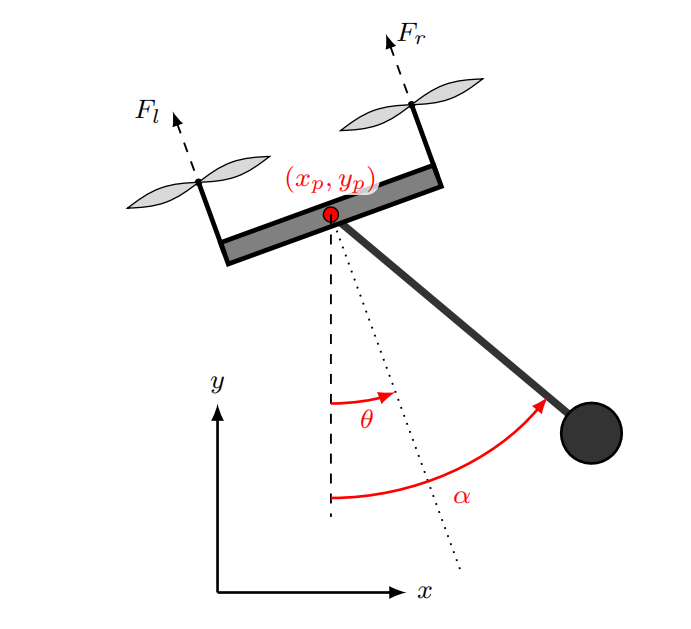
\includegraphics[scale=.54]{figs/quadrotor_model}
  \caption{Simplified quadrotor model}
\end{figure}

So we have:
\begin{equation}
     u_{0}=F_{s}
\end{equation}
\begin{equation}
     u_{1}=F_{d}
\end{equation}

where 
\begin{equation}
     F_{s}=F_{l}+F_{r}
\end{equation}
\begin{equation}
     F_{d}=F_{r}-F_{l}
\end{equation}

\section{Discretize the Dynamics}

The dynamic equations are discretized in the following way:
\begin{equation}
     x_{0,t+1}=x_{0,t}+\delta t[V_{x}]
\end{equation}
\begin{equation}
     x_{1,t+1}=x_{1,t}+\delta t[V_{y}]
\end{equation}
\begin{equation}
     x_{2,t+1}=x_{2,t}+\delta t[\omega_{\alpha}]
\end{equation}
\begin{equation}
     x_{3,t+1}=x_{3,t}+\delta t[\omega_{\theta}]
\end{equation}
\begin{equation}
     x_{4,t+1}=x_{4,t}+\delta t[\frac{m}{m+M}L(\omega_{\alpha})^{2}sin(\alpha)-\frac{F_{s}}{m+M}(sin(\theta)-\frac{m}{M}sin(\alpha-\theta)cos(\alpha))]
\end{equation}
\begin{equation}
     x_{5,t+1}=x_{5,t}+\delta t[-\frac{m}{m+M}L(\omega_{\alpha})^{2}cos(\alpha)+\frac{F_{s}}{m+M}(cos(\theta)+\frac{m}{M}sin(\alpha - \theta)sin(\alpha)-g)]
\end{equation}
\begin{equation}
     x_{6,t+1}=x_{6,t}+\delta t[-\frac{F_{s}}{ML}sin(\alpha - \theta)]
\end{equation}
\begin{equation}
     x_{7,t+1}=x_{7,t}+\delta t[\frac{lF_{d}}{J}]
\end{equation}
where:
\begin{itemize}
     \item[] $x_{0}$ represents the horizontal coordinates of the quadrotor at the current time t.
     \item[] $x_{1}$ represents the vertical coordinates of the quadrotor, the altitude y at the current time t.
     \item[] $x_{2}$ represents the angle of the pendulum $\alpha$ with respect to the inertial frame at the current time t.
     \item[] $x_{3}$ represents the the roll angle of the quadrotor $\theta$ at the current time t.
     \item[] $x_{4}$ represents the horizontal velocity of the quadrotor $V_{x}$ at the current time t.
     \item[] $x_{5}$ represents the vertical velocity of the quadrotor $V_{y}$ at the current time t.
     \item[] $x_{6}$ represents the angular velocity of the pendulum $\omega_{\alpha}$ at the current time t.
     \item[] $x_{7}$ represents the angular velocity of the quadrotor $\omega_{\theta}$ at the current time t.
     \item[] $\delta t$ represents the discretization time-step.
\end{itemize}

To apply Newton's Method, it is better to express the system dynamics as a vector field, as shown below. Subsequently, computing the first-order derivatives with respect to all states and inputs facilitates the derivation of the gradient for the method. And the discretized dynamic equations can be rewritten in the following form:
\\\begin{align*}
f(x,u)&=\begin{bmatrix}
						f_{1}(x,u)\\
                                f_{2}(x,u)\\
                                f_{3}(x,u)\\
                                f_{4}(x,u)\\
                                f_{5}(x,u)\\
                                f_{6}(x,u)\\
                                f_{7}(x,u)\\
                                f_{8}(x,u)\\
					 \end{bmatrix}=\begin{bmatrix}
                                             x_{0,t}+\delta t[V_{x}]\\
                                             x_{1,t}+\delta t[V_{y}]\\
                                             x_{2,t}+\delta t[\omega_{\alpha}]\\
                                             x_{3,t+1}=x_{3,t}+\delta t[\omega_{\theta}]\\
                                             x_{4,t}+\delta t[\frac{m}{m+M}L(\omega_{\alpha})^{2}sin(\alpha)-\frac{F_{s}}{m+M}(sin(\theta)-\frac{m}{M}sin(\alpha-\theta)cos(\alpha))]\\                              
                                             x_{5,t}+\delta t[-\frac{m}{m+M}L(\omega_{\alpha})^{2}cos(\alpha)+\frac{F_{s}}{m+M}(cos(\theta)+\frac{m}{M}sin(\alpha - \theta)sin(\alpha)-g)]\\
                                             x_{6,t}+\delta t[-\frac{F_{s}}{ML}sin(\alpha - \theta)]\\
                                             x_{7,t}+\delta t[\frac{lF_{d}}{J}]
                                            \end{bmatrix}
\\\end{align*}

\section{Get Equilibria}

We explored the equilibrium points of the quadrotor system by equating the vector field describing the system dynamics to zero. Due to the non-linear nature of the problem, multiple solutions exist. The simplest solution to get is the conditions for fixed position. So we get two equilibrium points from one fixed position to another fixed position which are $\mathbf{[ 0\ 0\ 0\ 0\ 0\ 0\ 0\ 0 ]}^\top$ and $\mathbf{[ 5\ 5\ 0\ 0\ 0\ 0\ 0\ 0 ]}^\top$. In this way we defined the Step trajectory of task 1.

For task 2, to generate a desired (smooth) state-input curve, we use the bell function to create a smooth reference curve from the state $\mathbf{[ 0\ 0\ 0\ 0\ 0\ 0\ 0\ 0 ]}^\top$ to the state $\mathbf{[ 5\ 5\ 0\ 0\ 0\ 0\ 0\ 0 ]}^\top$. 


%%%%%%%%%% Chapter Title %%%%%%%%%%
%%%%%%%%%%TASK 1 PROBELM SETUP%%%%%
\chapter{Task 1 - Trajectory generation (I)}
\section{Newton's Method with Affine Cost and Dynamics}

In this project we use the descent algorithm usually used in optimization which is called the Newton's Method. It is more efficient and at the same time more computationally expensive than the standard Gradient Method. Considering in same cases (especially at the first iterations) the matrices $Q_t^{k}$, $R_t^{k}$ and $S_t^{k}$ may not be positive definite, a different version of the algorithm will be applied which is called Newton's with affine cost and dynamics. This resembles a first-order method (with only first derivatives) so it will be faster.

And for each iteration, we are required to solve the following LQR problem to compute the descent direction $\Delta u_0$, ..., $\Delta u_{T-1}$.

\begin{equation*}
\begin{aligned}
\min_{\substack{{\Delta \tilde x_1,...,\Delta \tilde x_T}\\{\Delta u_0,...,\Delta u_T-1}}} \;  \sum\limits_{t=0}^{T-1}\frac{1}{2}\begin{bmatrix} \Delta \tilde x_t \\ \Delta u_t \end{bmatrix}^\top  \begin{bmatrix} \tilde Q_t & \tilde S_t^\top \\ \tilde S_t & \tilde R_t \end{bmatrix}\begin{bmatrix} \Delta \tilde x_t \\ \Delta u_t \end{bmatrix} +\frac{1}{2}\Delta \tilde x_T^\top Q_T\Delta \tilde x_T\\
\\\textrm{s.t.} \Delta \tilde x_{t+1}=\tilde A_t\Delta \tilde x_t+\tilde B_t\Delta u_t & \\
& \Delta \tilde x_0 \; given  \\
\end{aligned}
\end{equation*}
\\
This is a LQR optimal problem by augumenting the state as $\Delta \tilde x_t$ and rewriting the cos and system matrices as $\tilde Q_t$, $\tilde S_t$, $\tilde R_t$, $\tilde A_t$ and $\tilde B_t$.

Where,
\begin{itemize}
    \item $ \Delta \tilde x_t := \begin{bmatrix} 1 \\ \Delta x_t\end{bmatrix}$
    \item $ \tilde Q_t := \begin{bmatrix} 0 & q_t^\top \\ q_t & Q_t \end{bmatrix}$
    \item $ \tilde S_t := \begin{bmatrix} r_t & S_t \end{bmatrix}$
    \item $ \tilde R_t:= R_t $ 
    \item $ \tilde A_t:= \begin{bmatrix} 1 & 0 \\ c_t & A_t \end{bmatrix}$
    \item $ \tilde B_t:= \begin{bmatrix} 0 \\ B_t \end{bmatrix} $
\end{itemize}


During each iteration, it is necessary to calculate a series of matrices and vectors for solving the LQ problem with affine terms. This process involves working backward, commencing at time t=T while taking into account $P_T$ = $Q_T$ and $p_T$ = $q_T$.

Where,
\begin{itemize}
    \item $K^*_t = -(R_t+B_t^\top P_{t+1}B_t)^{-1}(S_t+B_t^\top P_{t+1}A_t)$
    \item $\sigma^*_t = -(R_t+B_t^\top P_{t+1}B_t)^{-1}(r_t+B_t^\top p_{t+1}+B_t^\top P_{t+1}c_t)$
    \item $p_t = q_t+A_t^\top p_{t+1}+A_t^\top P_{t+1}c_t+{K^*_t}^\top (R_t+B_t^\top P_{t+1}B_t) \sigma^*_t$
    \item $P_t = Q_t+A_t^\top P_{t+1}A_t-{K^*_t}^\top (R_t+B_t^\top P_{t+1}B_t)K^*_t$
\end{itemize}

And the optimal solution of the problem reads
\begin{equation*}
\begin{aligned}
\Delta u^*_t=K^*_t\Delta x^*_t+\sigma^*_t
\end{aligned}
\end{equation*}
\begin{equation*}
\begin{aligned}
\Delta x^*_{t+1}=A_t\Delta x^*_t+B_t\Delta u^*_t
\end{aligned}
\end{equation*}

At the same time we need to update the input trajectory as following:
\begin{equation*}
\begin{aligned}
u_t^{k+1}=u_t^{k}+\gamma^{k}(\sigma_t^k+K_t^{k}\Delta x^{k}_t)\approx u_t^{k}+\gamma^{k}(\sigma_t^k+K_t^{k}(x_t^{t+1}-x_t^{k}))
\end{aligned}
\end{equation*}

where $\gamma^{k}$ is the step-size chosen by Armijo rule.

\section{Step Function}

In this task, we try to define a Step function between two equilibrium points for the trajectory of the quadrotor. The Step Function is generated by the file \texttt{step\_reference} that simply takes constant values of the horizontal coordinate $x_{p}=0$, the vertical coordinate $y_{p}=0$ and the first input $F_{s}=0$ for $ t = \{1, 2, ..., \frac{T}{2}\}$ as well as the horizontal coordinate $x_{p}=5$, the vertical coordinate $y_{p}=5$ and the first input $F_{s}=(m+M)g$ for $ t = \{\frac{T}{2}+1, ..., T\}$. The Step Function jumps from the two levels can be defined as following:

$$ x_{p}=\left\{
\begin{aligned}
x_{p}=0  \;\;\;\;\;for\;\;\;\;\;   t = \{0, 1, 2, ..., \frac{T}{2}\}\\
x_{p}=5   \;\;\;\;\;for\;\;\;\;\;   t = \{\frac{T}{2}+1, ..., T\}
\end{aligned}
\right.
$$

$$ y_{p}=\left\{
\begin{aligned}
y_{p}=0  \;\;\;\;\;for\;\;\;\;\;   t = \{0, 1, 2, ..., \frac{T}{2}\}\\
y_{p}=5   \;\;\;\;\;for\;\;\;\;\;   t = \{\frac{T}{2}+1, ..., T\}
\end{aligned}
\right.
$$

$$ F_{s}=\left\{
\begin{aligned}
F_{s}=0  \;\;\;\;\;for\;\;\;\;\;   t = \{0, 1, 2, ..., \frac{T}{2}\}\\
F_{s}=(m+M)g   \;\;\;\;\;for\;\;\;\;\;   t = \{\frac{T}{2}+1, ..., T\}
\end{aligned}
\right.
$$

\begin{equation}
    x^{des}_{0,t+1}=x_{p}
\end{equation}
\begin{equation}
    x^{des}_{1,t+1}=y_{p}
\end{equation}
\begin{equation}
    x^{des}_{2,t+1}=0
\end{equation}
\begin{equation}
    x^{des}_{3,t+1}=0
\end{equation}
\begin{equation}
    x^{des}_{4,t+1}=0
\end{equation}
\begin{equation}
    x^{des}_{5,t+1}=0
\end{equation}
\begin{equation}
    x^{des}_{6,t+1}=0
\end{equation}
\begin{equation}
    x^{des}_{7,t+1}=0
\end{equation}
\begin{equation}
    u^{des}_{0,t+1}=F_{s}
\end{equation}
\begin{equation}
    u^{des}_{1,t+1}=0
\end{equation}

\begin{figure}[H]
  \begin{minipage}{\linewidth}
  \centering
  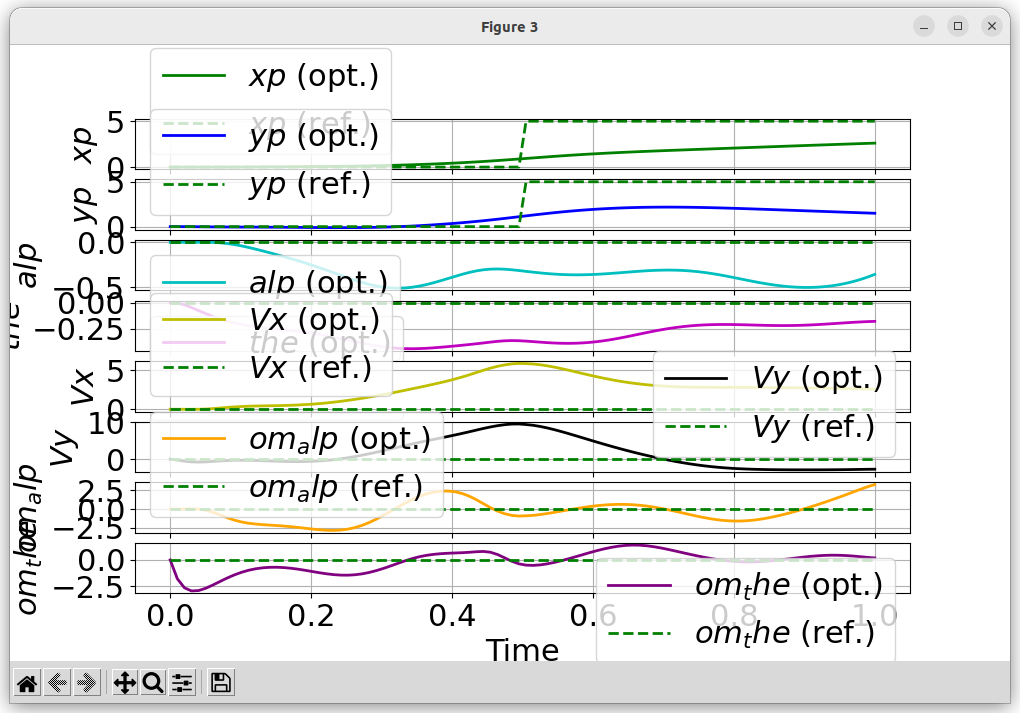
\includegraphics[width=1\textwidth]{figs/Optimal traj and desired curve iteration-5}
  \end{minipage}
  \caption{Optmal trajectory and desired curve iteration-5}
\end{figure}
\begin{figure}[H]
  \begin{minipage}{\linewidth}
  \centering
  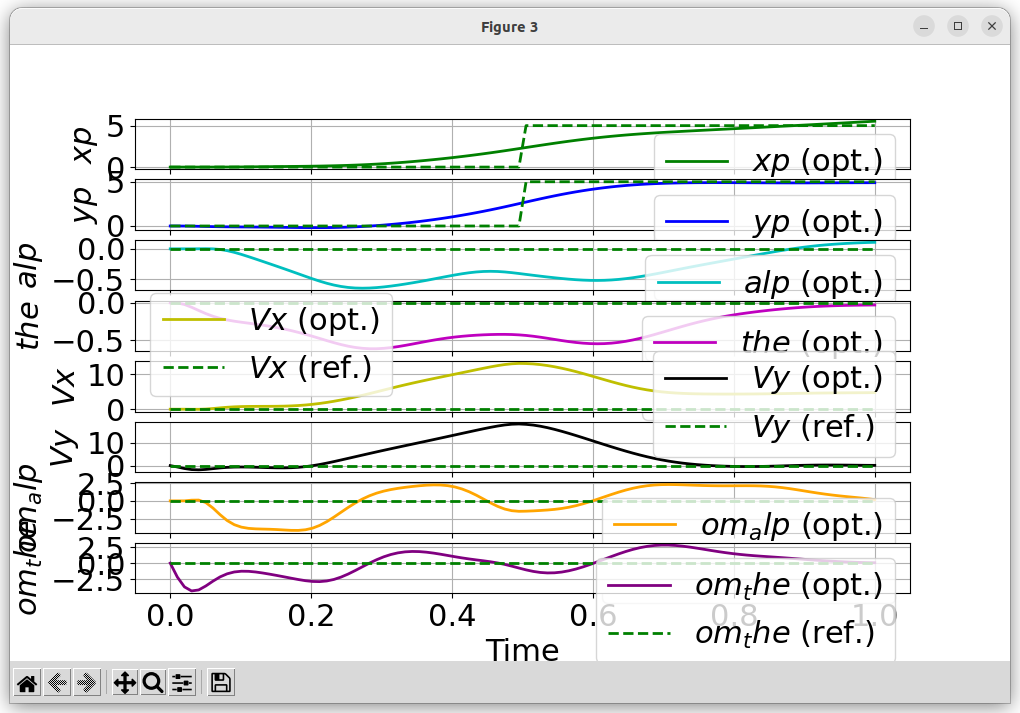
\includegraphics[width=1\textwidth]{figs/Optimal traj and desired curve final}
  \end{minipage}
  \caption{Optmal trajectory and desired curve final}
\end{figure}
\begin{figure}[H]
  \begin{minipage}{\linewidth}
  \centering
  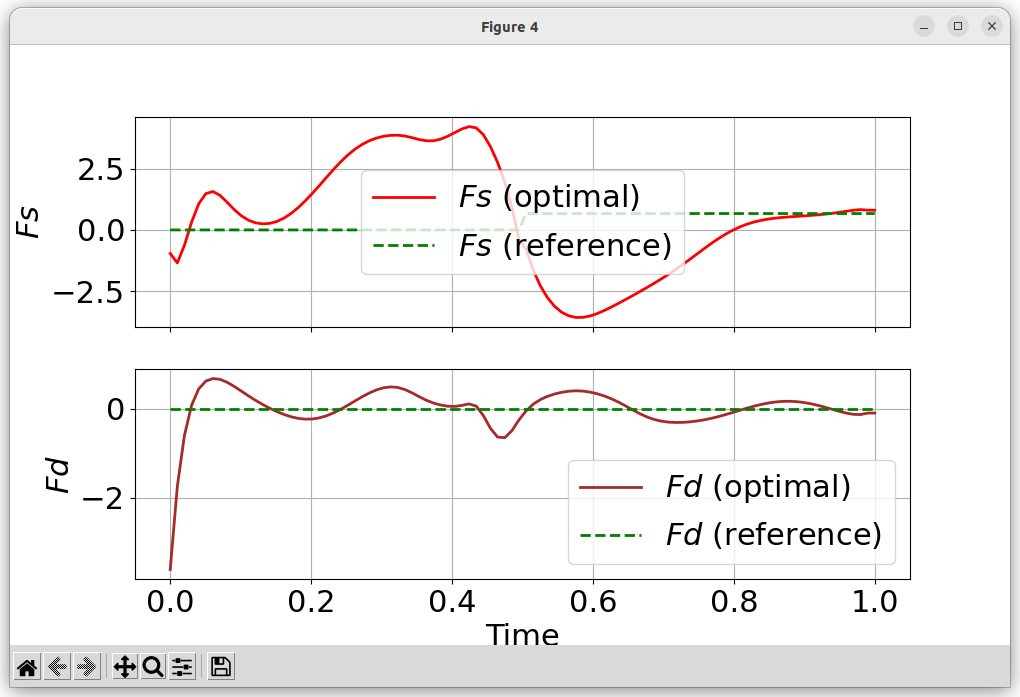
\includegraphics[width=1\textwidth]{figs/Optimal traj and desired curve for inputs final}
  \end{minipage}
  \caption{Optimal trajectory for inputs and desired input curve}
\end{figure}

As shown in Figure 2.1-2.3: the dotted lines represent the step trajectory that we defined (the reference trajectory) and the solid lines represent the optimal trajectory computed by the Newton's Method.

\begin{figure}[H]
  \begin{minipage}{\linewidth}
  \centering
  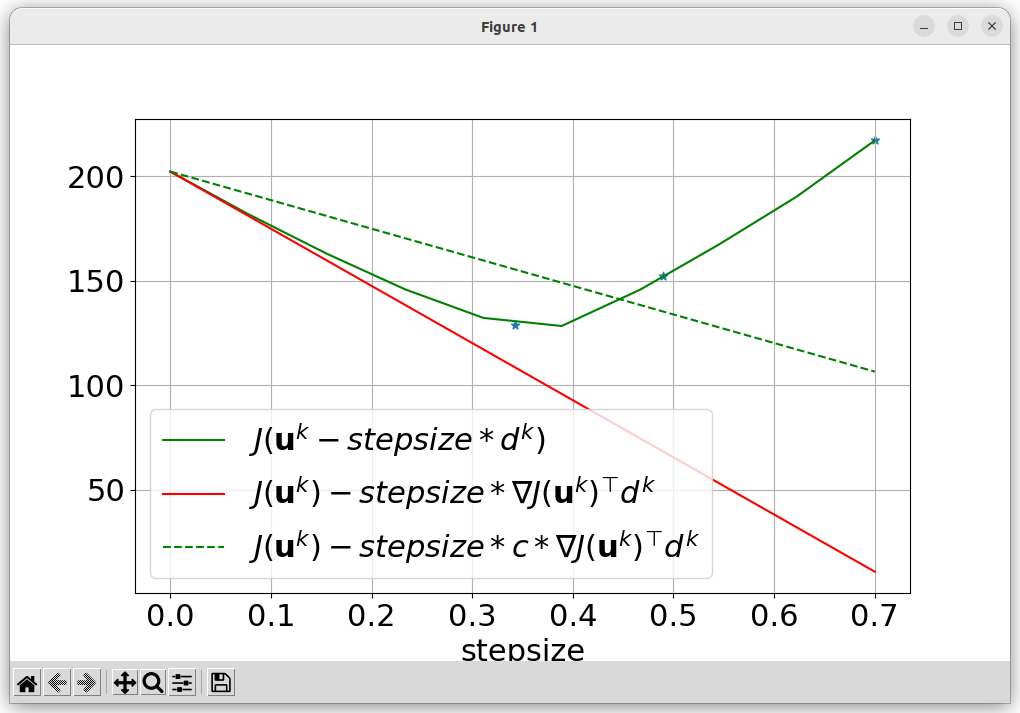
\includegraphics[width=1\textwidth]{figs/Armijo descent direction plot at iteration-1}
  \end{minipage}
  \caption{Armijo descent direction plot iteration-1}
\end{figure}
\begin{figure}[H]
  \begin{minipage}{\linewidth}
  \centering
  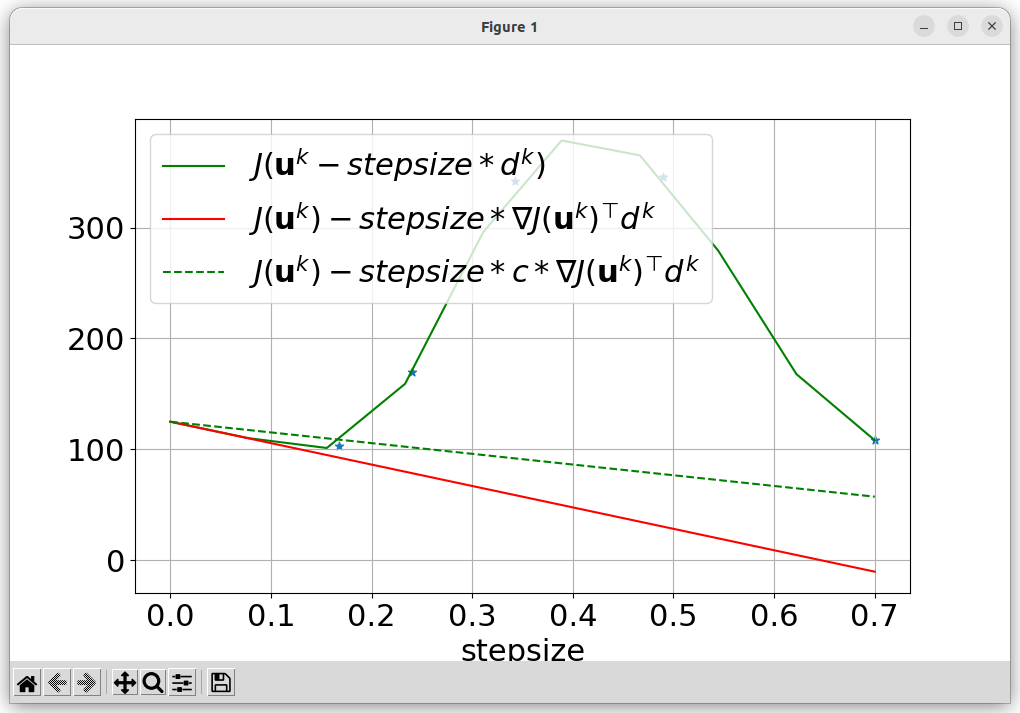
\includegraphics[width=1\textwidth]{figs/Armijo descent direction plot at iteration-3}
  \end{minipage}
  \caption{Armijo descent direction plot iteration-3}
\end{figure}
\begin{figure}[H]
  \begin{minipage}{\linewidth}
  \centering
  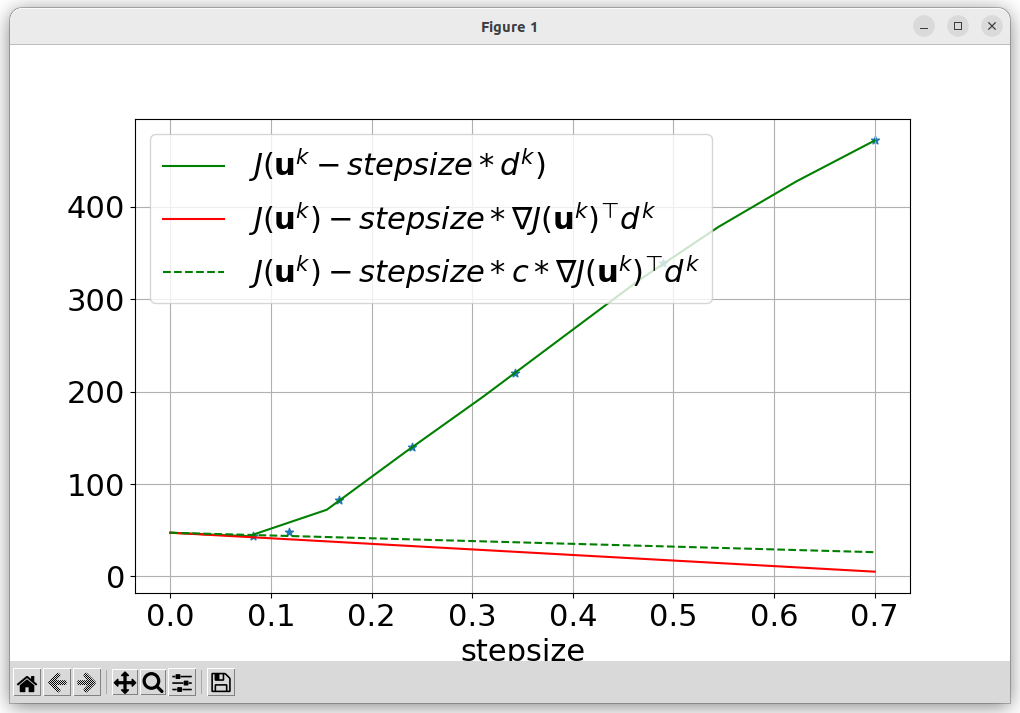
\includegraphics[width=1\textwidth]{figs/Armijo descent direction plot at iteration-5}
  \end{minipage}
  \caption{Armijo descent direction plot iteration-5}
\end{figure}
\begin{figure}[H]
  \begin{minipage}{\linewidth}
  \centering
  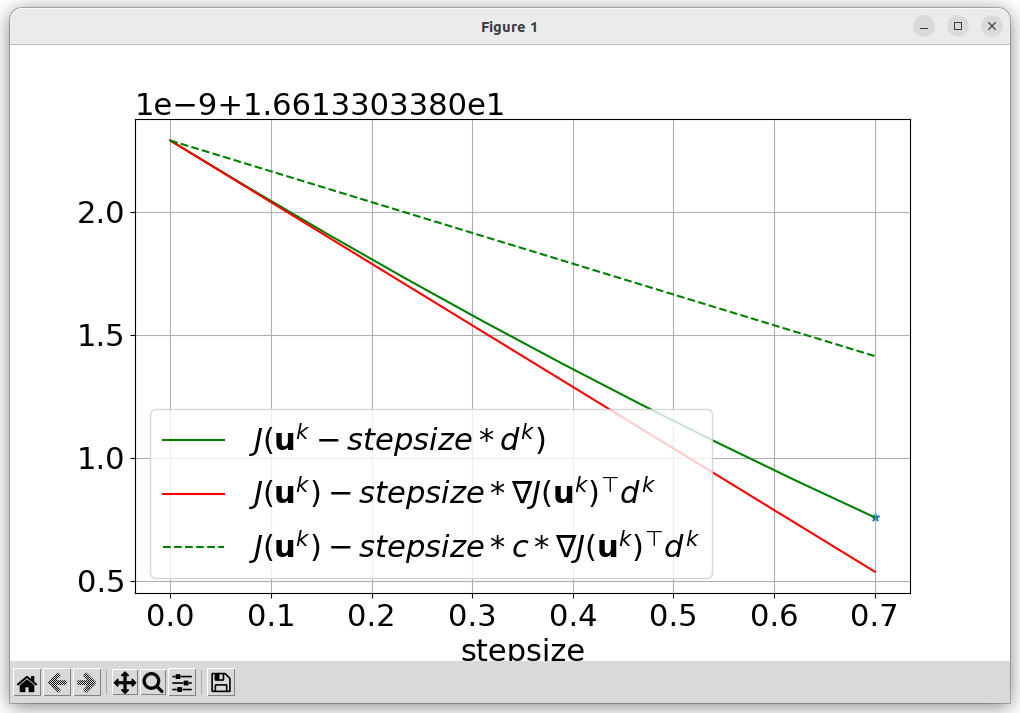
\includegraphics[width=1\textwidth]{figs/Armijo descent direction plot at last iterations}
  \end{minipage}
  \caption{Armijo descent direction plot final}
\end{figure}

The final Armijo's selection rule and its iterations for the our Step function are shown in Figure 2.4-2.7.

\begin{figure}[H]
  \begin{minipage}{\linewidth}
  \centering
  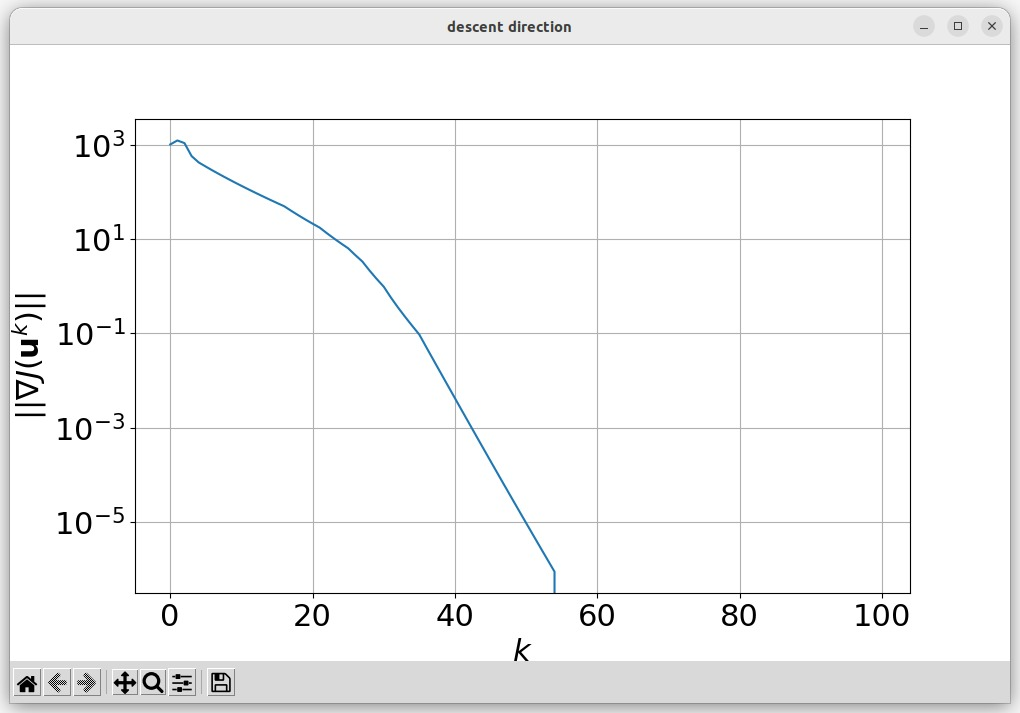
\includegraphics[width=1\textwidth]{figs/Norm of the Descent Direction-1}
  \end{minipage}
  \caption{Norm of the Descent Direction}
\end{figure}

Figure 2.8 illustrates the descent direction norm for the Step trajectory. In this particular test, we established a maximum iteration limit of 100. As depicted in the plot, the descent direction norm consistently diminishes throughout the iterations. This observation indicates that our optimizer is functioning appropriately, steadily approaching the minimum.

\begin{figure}[H]
  \begin{minipage}{\linewidth}
  \centering
  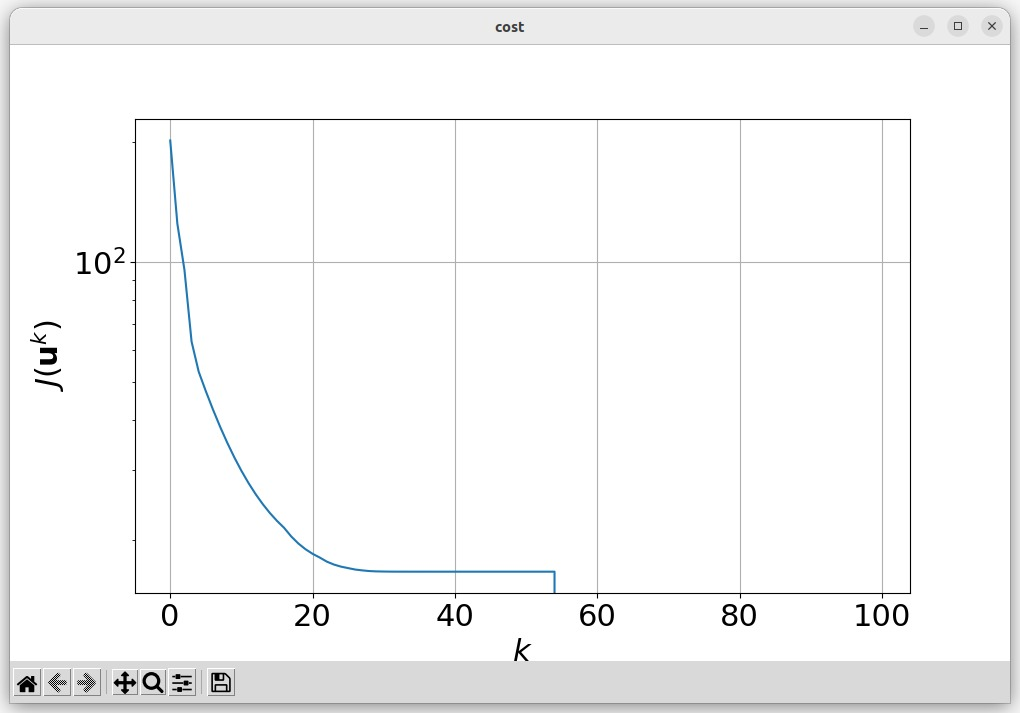
\includegraphics[width=1\textwidth]{figs/Cost of the Step Trajectory}
  \end{minipage}
  \caption{Cost of the Step Trajectory}
\end{figure}

The Cost Function continuously decreases over the course of all 54 iterations, which is a positive outcome given that our objective is to minimize it.

\chapter{Task 2 - Trajectory generation (II)}
\section{Bell-Shaped Reference Trajectory}

In task 2, we need to generate a desired (smooth) state-input curve. As a result, we use the function \texttt{reference\_curve} to define a bell-shaped trajectory. The first input $F_{s}$ will be increased from 0 to (m+M)g in a smooth curve (bell-function). And meanwhile the first two states will also be increased from $\mathbf{[ 0\ 0 ]}^\top$ to $\mathbf{[ 5\ 5 ]}^\top$ in the same smooth curve (bell-function).

It should be emphasized that the trajectory with a bell-shaped curve is inherently smooth, as we utilize its mathematical definition to calculate the reference values for optimization. Here are the behaviours of the generated trajectory:

\begin{figure}[H]
  \begin{minipage}{\linewidth}
  \centering
  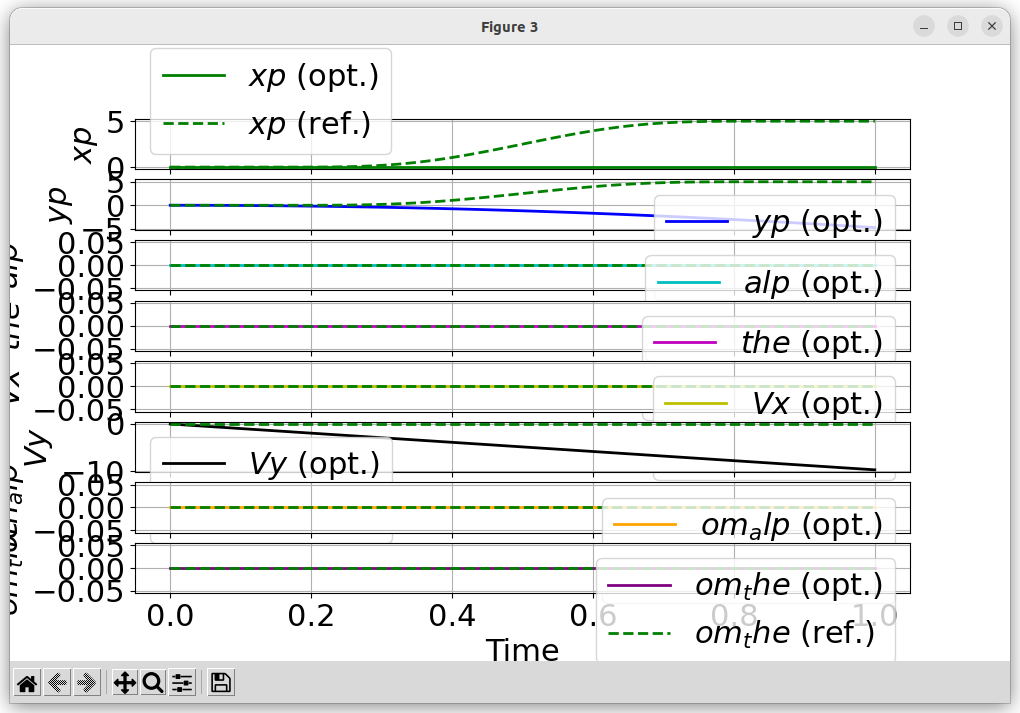
\includegraphics[width=1\textwidth]{figs/optmal trajectory and desired curve iteration-1}
  \end{minipage}
  \caption{Optmal trajectory and desired curve iteration-1}
\end{figure}
\begin{figure}[H]
  \begin{minipage}{\linewidth}
  \centering
  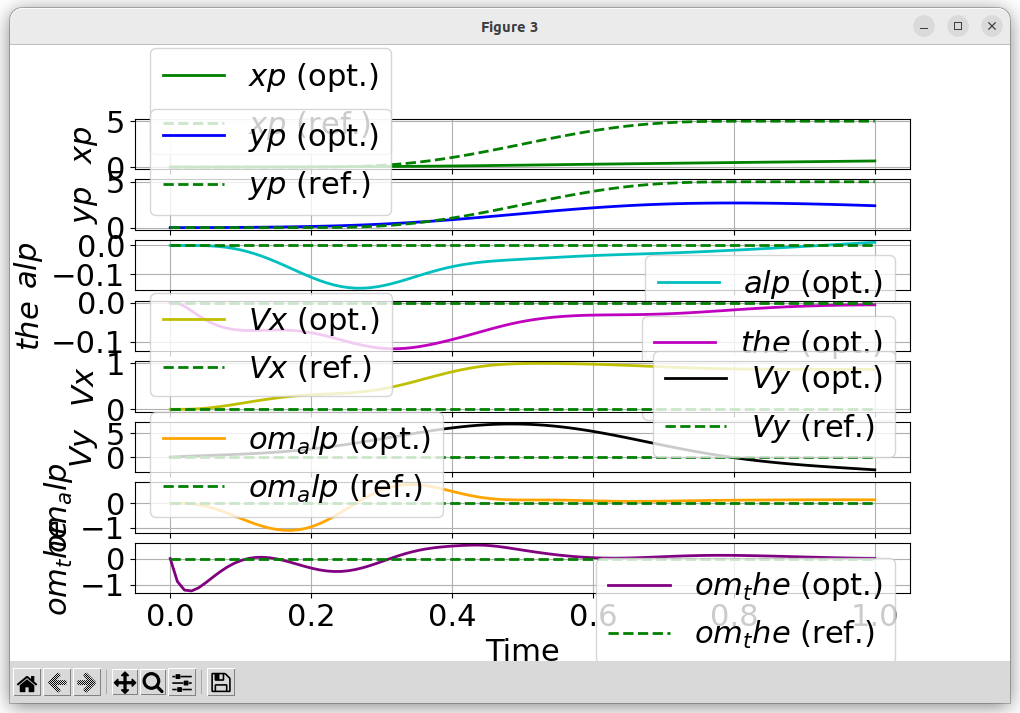
\includegraphics[width=1\textwidth]{figs/optmal trajectory and desired curve iteration-2}
  \end{minipage}
  \caption{Optmal trajectory and desired curve iteration-3}
\end{figure}
\begin{figure}[H]
  \begin{minipage}{\linewidth}
  \centering
  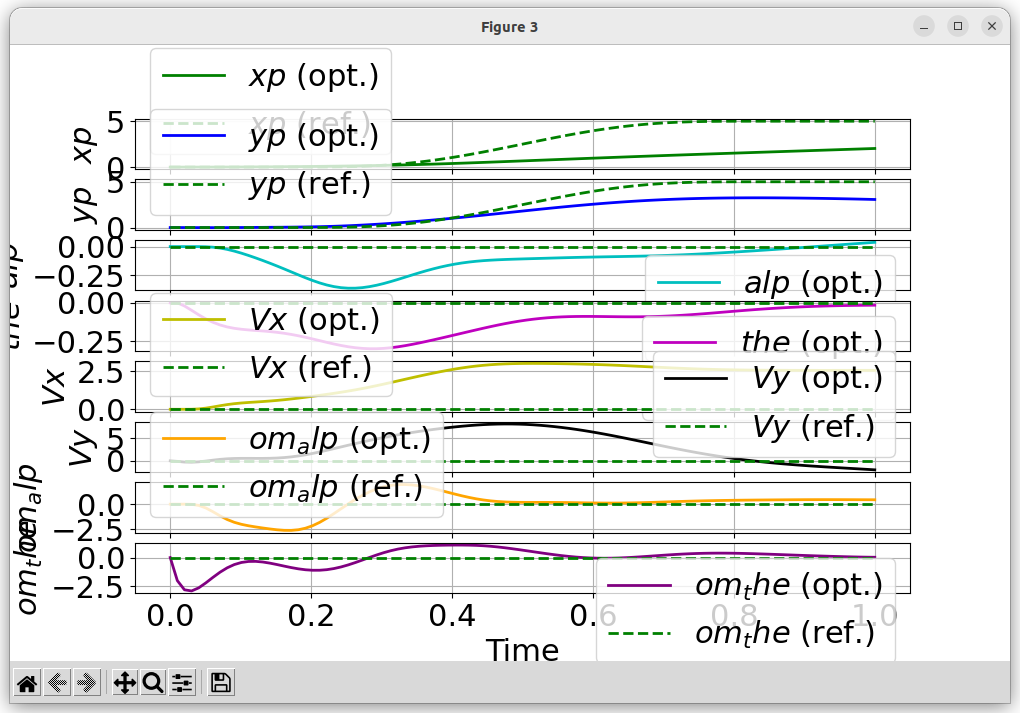
\includegraphics[width=1\textwidth]{figs/optmal trajectory and desired curve iteration-3}
  \end{minipage}
  \caption{Optmal trajectory and desired curve iteration-5}
\end{figure}
\begin{figure}[H]
  \begin{minipage}{\linewidth}
  \centering
  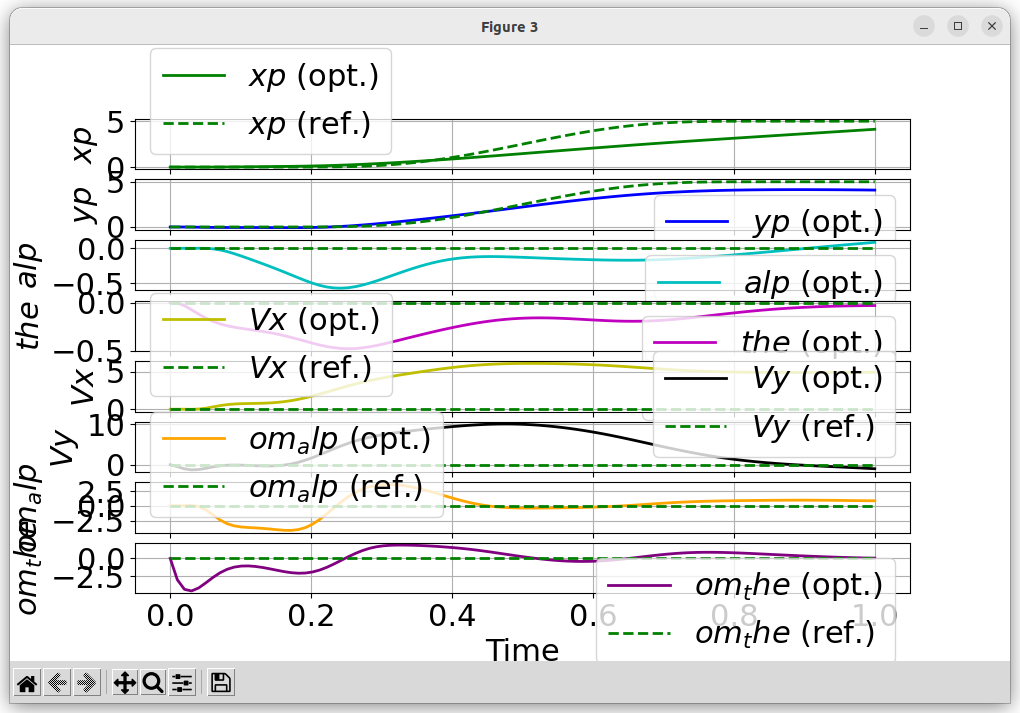
\includegraphics[width=1\textwidth]{figs/optmal trajectory and desired curve iteration-4}
  \end{minipage}
  \caption{Optmal trajectory and desired curve iteration-7}
\end{figure}
\begin{figure}[H]
  \begin{minipage}{\linewidth}
  \centering
  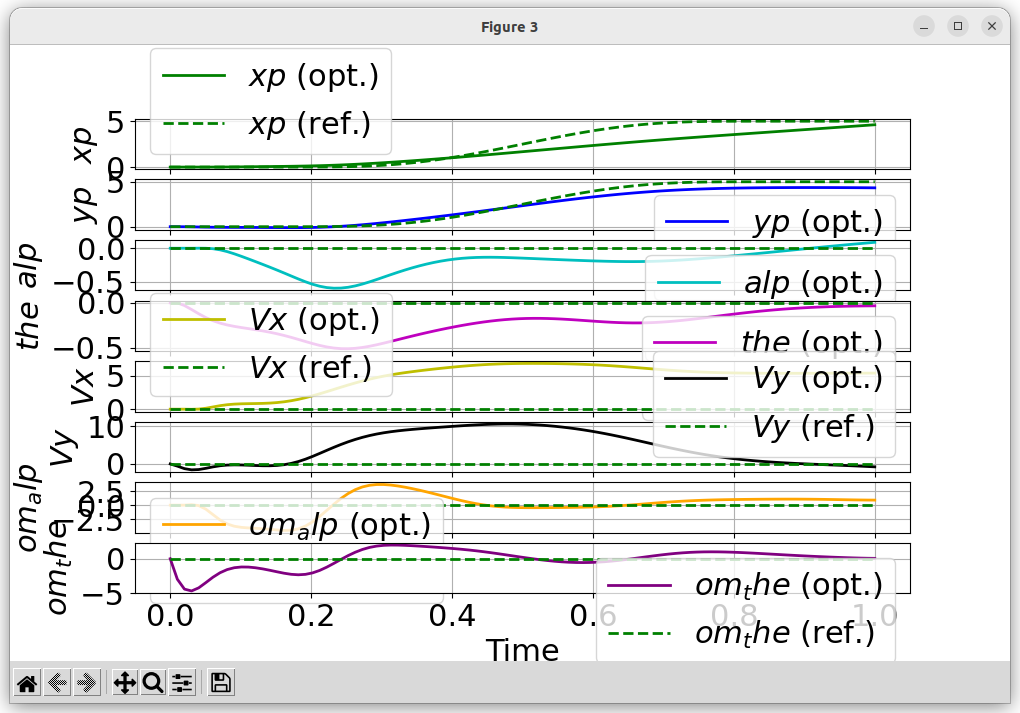
\includegraphics[width=1\textwidth]{figs/optmal trajectory and desired curve iteration-5}
  \end{minipage}
  \caption{Optmal trajectory and desired curve iteration-9}
\end{figure}
\begin{figure}[H]
  \begin{minipage}{\linewidth}
  \centering
  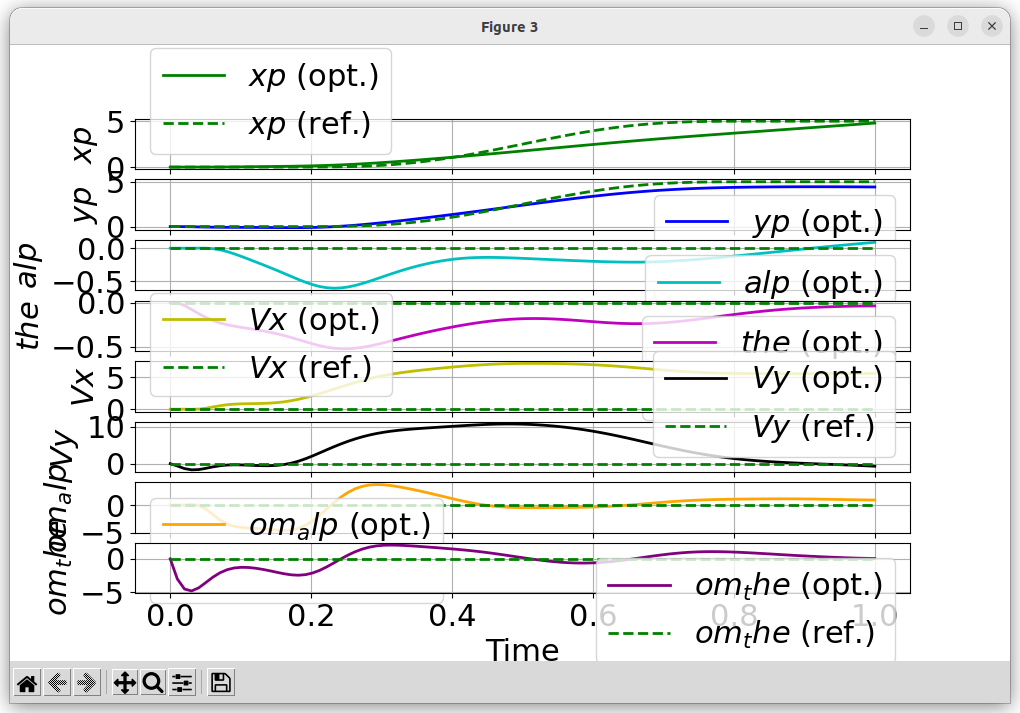
\includegraphics[width=1\textwidth]{figs/optmal trajectory and desired curve iteration-6}
  \end{minipage}
  \caption{Optmal trajectory and desired curve iteration-10}
\end{figure}
\begin{figure}[H]
  \begin{minipage}{\linewidth}
  \centering
  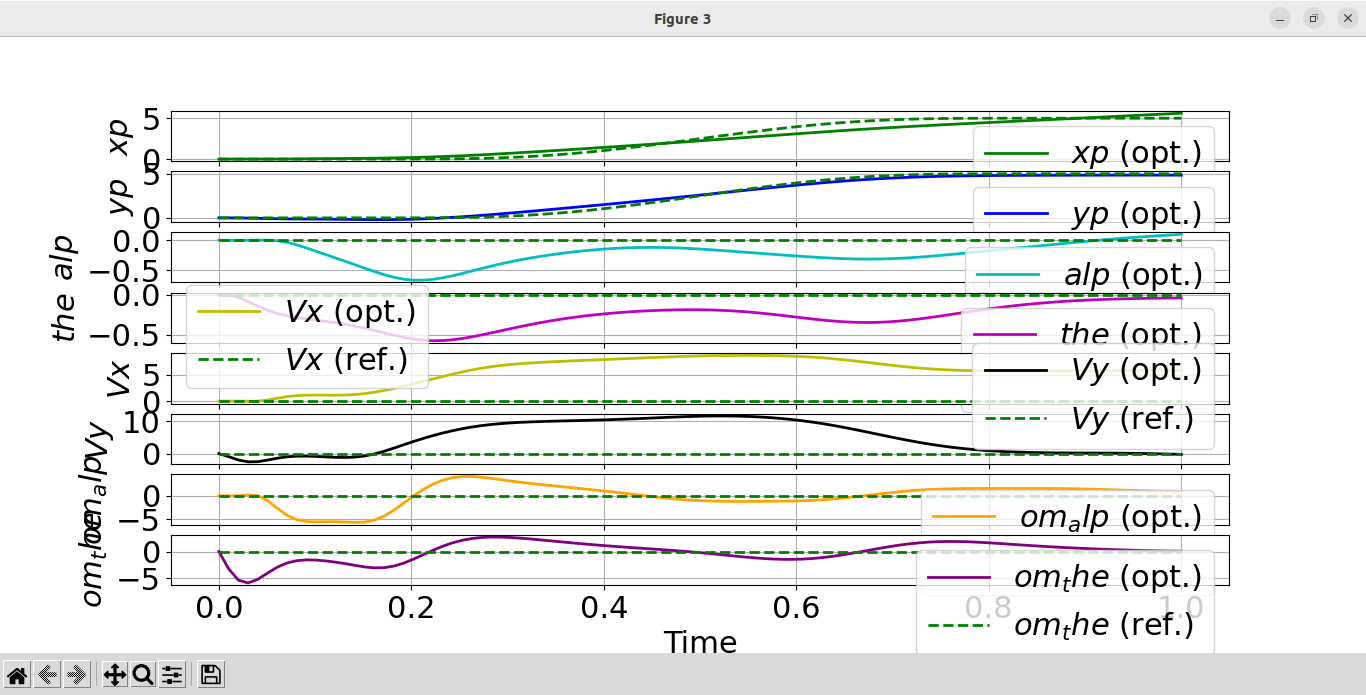
\includegraphics[width=1\textwidth]{figs/Optimal trajectory and desired curve final}
  \end{minipage}
  \caption{Optmal trajectory and desired curve fianl}
\end{figure}
\begin{figure}[H]
  \begin{minipage}{\linewidth}
  \centering
  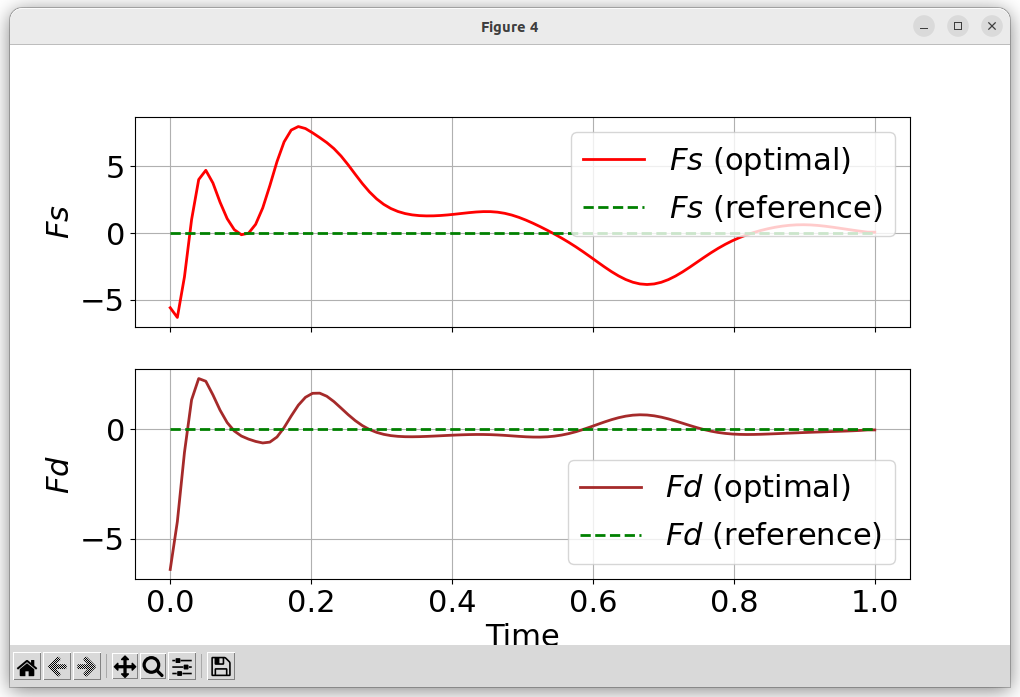
\includegraphics[width=1\textwidth]{figs/Optimal trajectory for inputs and desired input curve}
  \end{minipage}
  \caption{Optimal trajectory for inputs and desired input curve}
\end{figure}

As shown in Figure 3.1-3.8: the dotted lines represent the bell-shaped trajectory that we defined (the reference trajectory) and the solid lines represent the optimal trajectory computed by the Newton's Method.

\begin{figure}[H]
  \begin{minipage}{\linewidth}
  \centering
  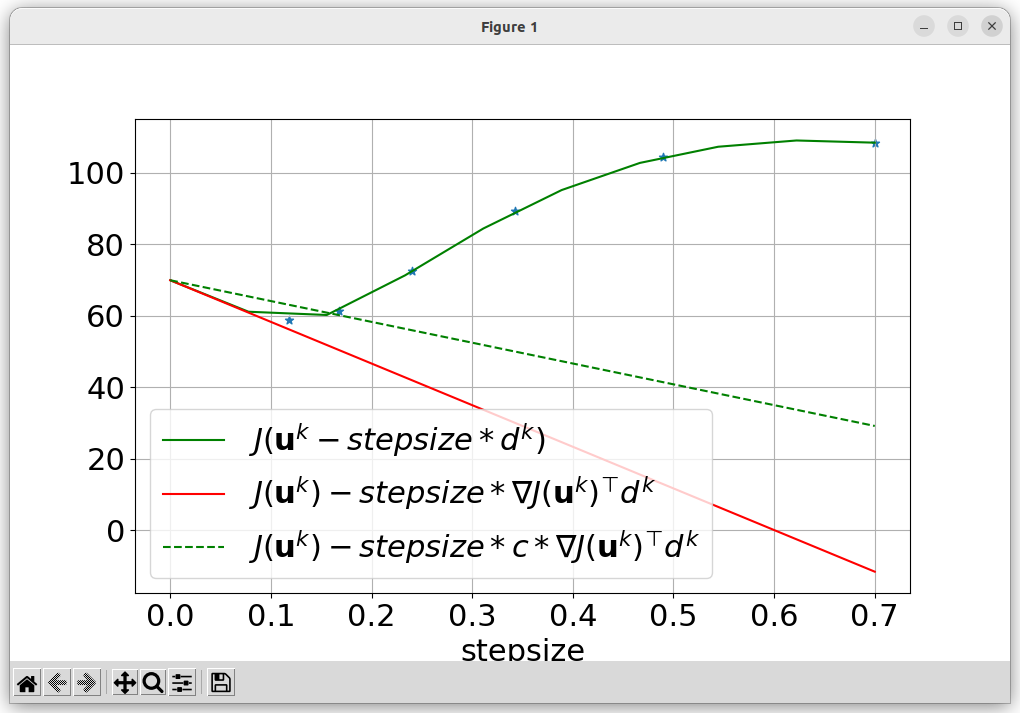
\includegraphics[width=1\textwidth]{figs/Armijo descent direction plot iteration-1}
  \end{minipage}
  \caption{Armijo descent direction plot iteration-1}
\end{figure}
\begin{figure}[H]
  \begin{minipage}{\linewidth}
  \centering
  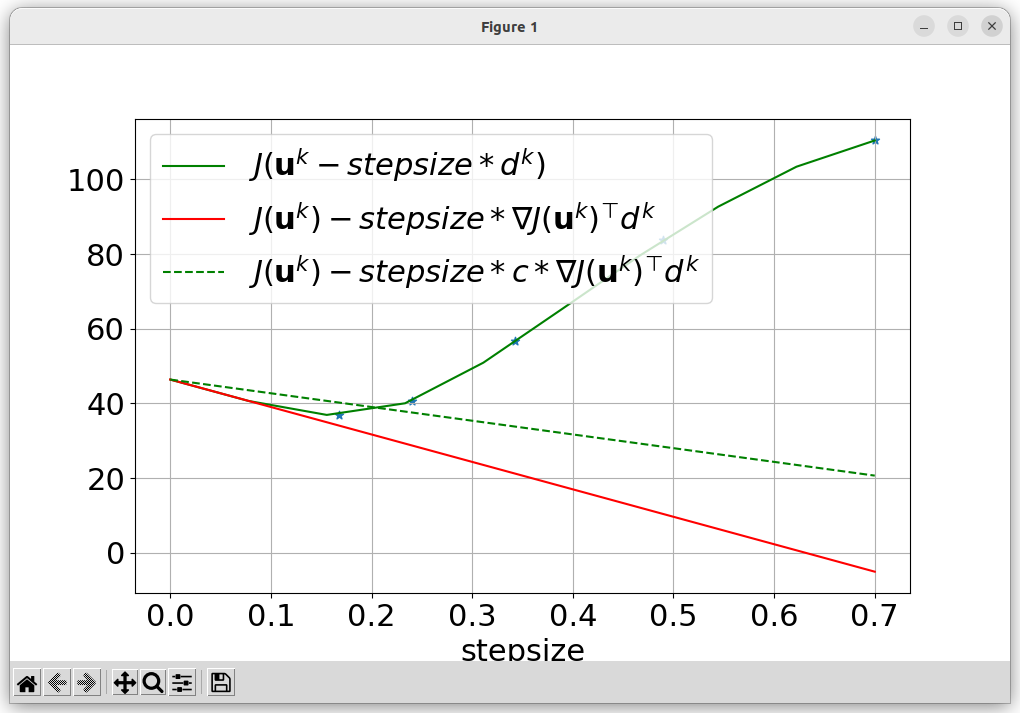
\includegraphics[width=1\textwidth]{figs/Armijo descent direction plot iteration-2}
  \end{minipage}
  \caption{Armijo descent direction plot iteration-3}
\end{figure}
\begin{figure}[H]
  \begin{minipage}{\linewidth}
  \centering
  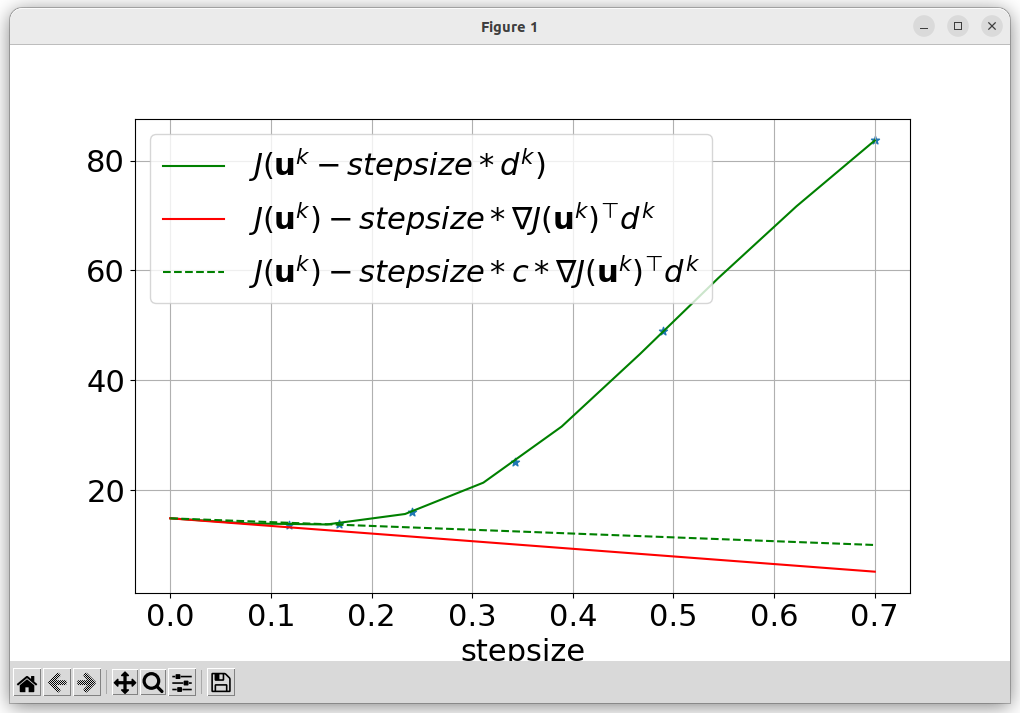
\includegraphics[width=1\textwidth]{figs/Armijo descent direction plot iteration-3}
  \end{minipage}
  \caption{Armijo descent direction plot iteration-5}
\end{figure}
\begin{figure}[H]
  \begin{minipage}{\linewidth}
  \centering
  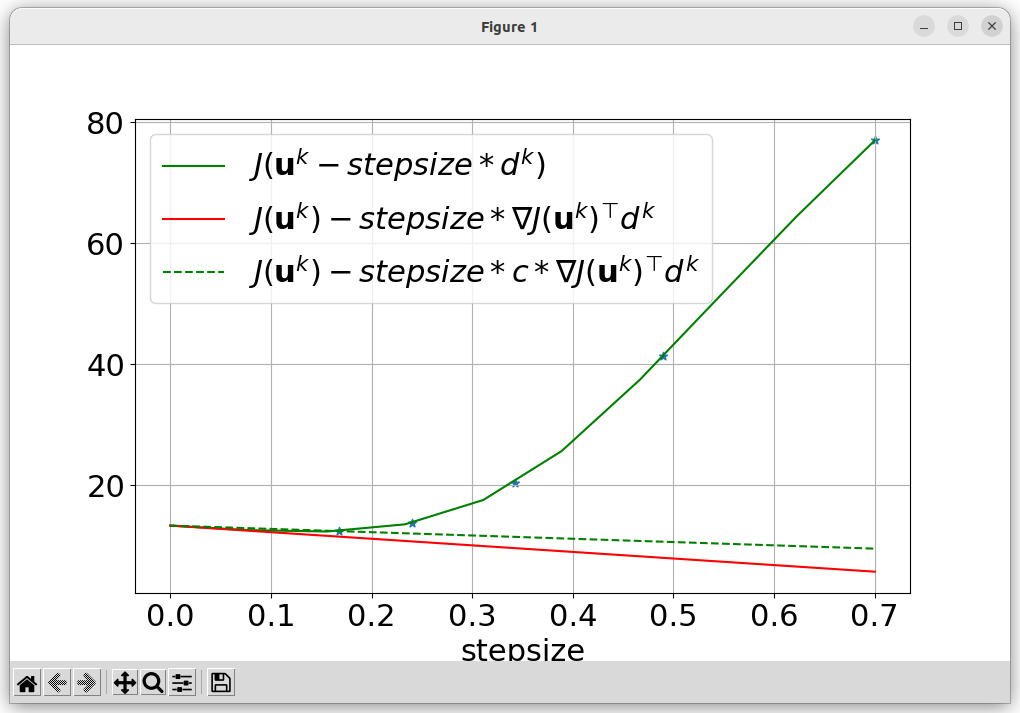
\includegraphics[width=1\textwidth]{figs/Armijo descent direction plot iteration-4}
  \end{minipage}
  \caption{Armijo descent direction plot iteration-7}
\end{figure}
\begin{figure}[H]
  \begin{minipage}{\linewidth}
  \centering
  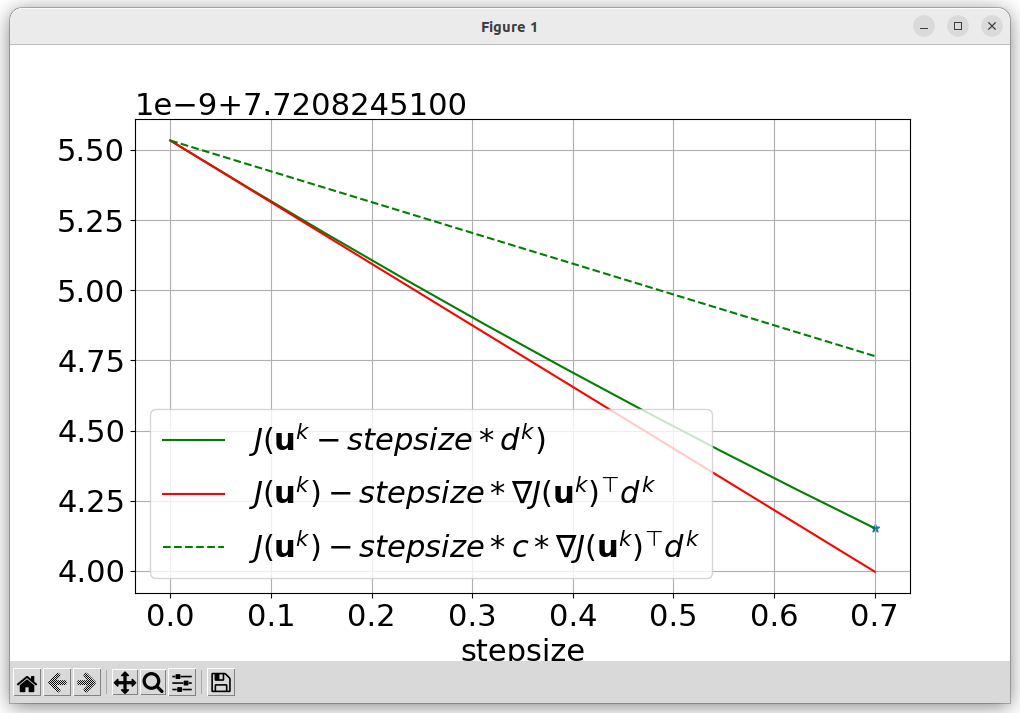
\includegraphics[width=1\textwidth]{figs/Armijo descent direction plot final}
  \end{minipage}
  \caption{Armijo descent direction plot final}
\end{figure}

The final Armijo's selection rule and its iterations for the our smooth function are shown in Figure 3.9-3.13.

\begin{figure}[H]
  \begin{minipage}{\linewidth}
  \centering
  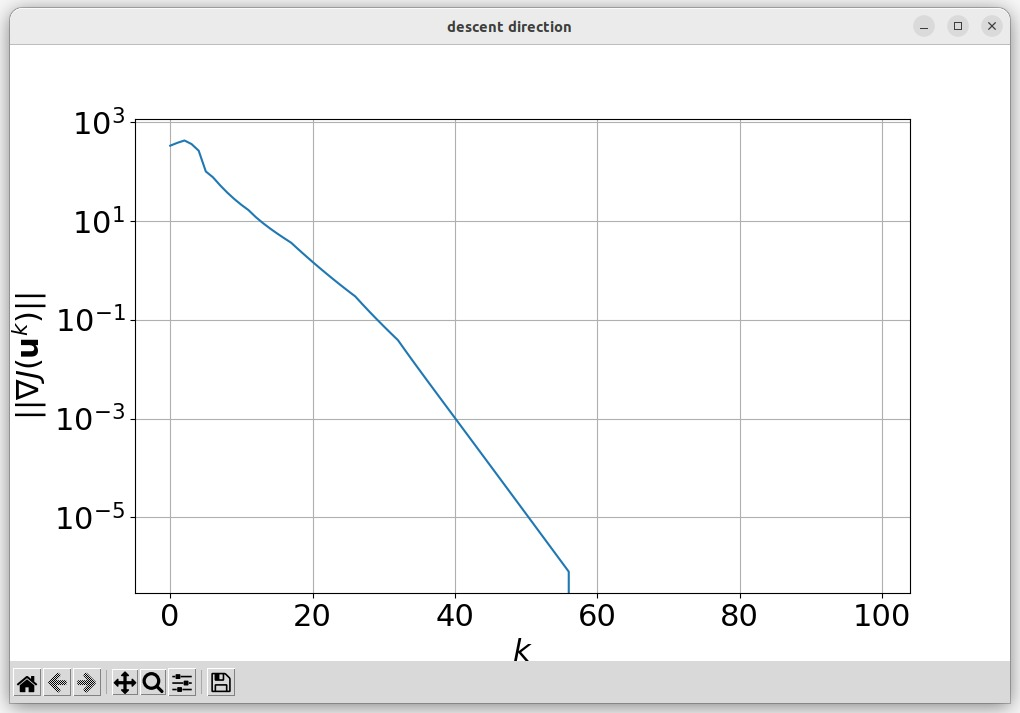
\includegraphics[width=1\textwidth]{figs/Norm of the Descent Direction-2}
  \end{minipage}
  \caption{Norm of the Descent Direction}
\end{figure}

Figure 3.14 illustrates the descent direction norm for the Bell-shaped trajectory. In this particular test, we established a maximum iteration limit of 100. As depicted in the plot, the descent direction norm consistently diminishes throughout the iterations. This observation indicates that our optimizer is functioning appropriately, steadily approaching the minimum.

\begin{figure}[H]
  \begin{minipage}{\linewidth}
  \centering
  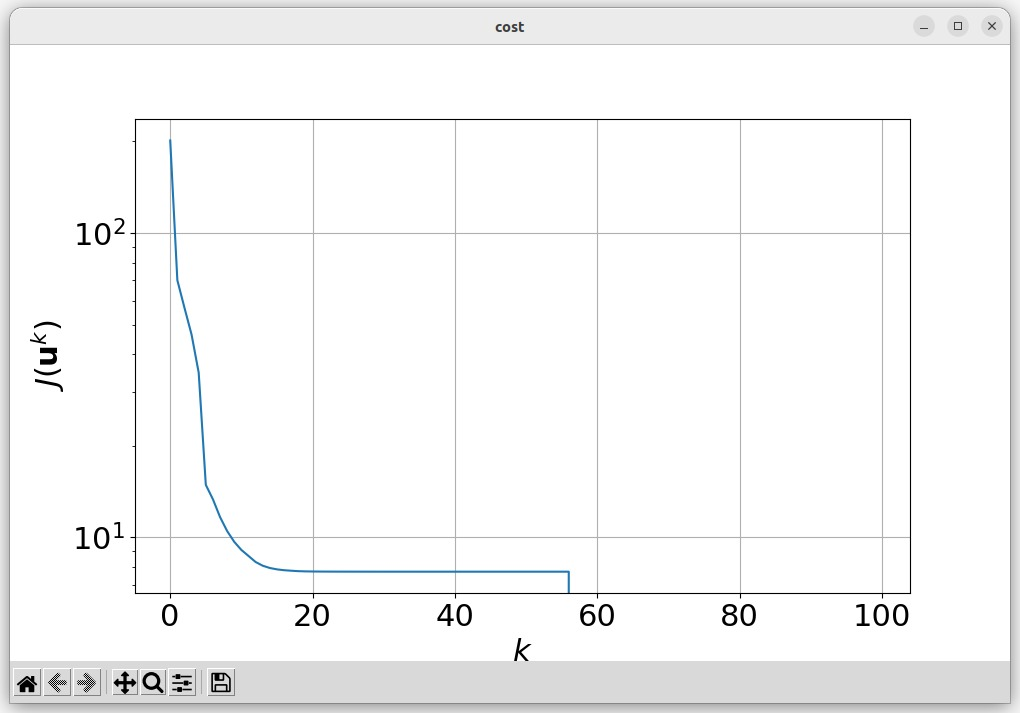
\includegraphics[width=1\textwidth]{figs/Cost of the Bell-shaped Trajectory}
  \end{minipage}
  \caption{Cost of the Bell-shaped Trajectory}
\end{figure}

The Cost Function continuously decreases over the course of all 56 iterations, which is a positive outcome given that our objective is to minimize it.

\chapter{Task 3 - Trajectory tracking via LQR}
\section{Tracking via LQR}

Idea: We want to use a (stablizing) feedback Linear Quadratic Regulator (LQR) on the linearization to track the optimal trajectory $(x^{opt},u^{opt})$.\\
\\
\textbf{Step 1: Linearize the dynamics about the optimal trajectory $(x^{opt},u^{opt})$ to get the LTV system }\\
\begin{equation*}
\Delta x_{t+1}= A_t^{opt}\Delta x_t + B_t^{opt}\Delta u_t \\
\end{equation*}

where $A_t^{opt} \in \mathbb{R}^{n \times n}$ and  $B_t^{opt} \in \mathbb{R}^{n \times m}$ are defined as:\\
\begin{equation*}
A_t^{opt} = \nabla_{1}f{(x_t^{opt},u_t^{opt})}^\top
\end{equation*}
\begin{equation*}
B_t^{opt} = \nabla_{2}f{(x_t^{opt},u_t^{opt})}^\top
\end{equation*}
\\
\textbf{Step 2: Calculate the LQ optimal feedback controller}\\

 Solving the optimal control problem
\begin{equation*}
\min_{\substack{{\Delta x_1,...,\Delta x_T}\\{\Delta u_0,...,\Delta u_T-1}}} \;  \sum\limits_{t=0}^{T-1}\Delta x_t^\top Q^{reg}_{t}\Delta x_t + \Delta u_t^\top R^{reg}_{t}\Delta u_t + \Delta x_T^\top Q^{reg}_{T}\Delta x_T\\
\end{equation*}
\begin{equation*}
\textrm{subj. to }\Delta x_{t+1}=A_t^{opt}\Delta x_t+B_t^{opt}\Delta u_t\;\;\;\;\;\;t=0,...,T-1\\
\end{equation*}
\begin{equation*}
\Delta x_{0} = 0
\end{equation*}

for some cost matrices $Q^{reg}_{t} \geq 0 \in \mathbb{R}^{n \times n}, ^{reg}_{t}> 0 \in \mathbb{R}^{n \times m}$ and $Q^{reg}_{T} \geq 0 \in \mathbb{R}^{n \times n} (degree \, of freedom).$ 

Set $P_T = Q^{reg}_{T}$ and backward iterate t = \{T-1, ..., 0\}:

\begin{equation*}
P_t=Q^{reg}_{t}+{A_t^{opt}}^\top P_{t+1}A_t^{opt} - ({A_t^{opt}}^\top P_{t+1}B_t^{opt})(R^{reg}_{t}+{B_t^{opt}}^\top P_{t+1}B_t^{opt})^{-1}({B_t^{opt}}^\top P_{t+1}A_t^{opt})
\end{equation*}

and define for all t = \{0, ..., T-1\}, compute the feedback gain $K^{reg}_{t} \in \mathbb{R}^{m \times n}$
\begin{equation*}
K^{reg}_{t}:= -(R^{reg}_{t} + {B_t^{opt}}^\top P_{t+1}B_t^{opt})^{-1}({B_t^{opt}}^\top P_{t+1}A_t^{opt})
\end{equation*}
\\
\textbf{Step 3: Track the generated (optimal) trajectory }\\

We apply the feedback controller designed on the linearization to the nonlinear system to track $(x^{opt},u^{opt})$. Namely for all t = \{0, ..., T-1\}, we apply 
\begin{equation*}
u_t=u_t^{opt}+K^{reg}_{t}(x_t - x_t^{opt})
\end{equation*}
\begin{equation*}
x_{t+1} = f(x_t,u_t)
\end{equation*}
\begin{equation*}
\textrm{with } x_0 = 0
\end{equation*}

Finally we get the tracked trajectory $(x^{lqr},u^{opt})$.\\

\section{Tracked Trajectories}

The controller monitors the trajectories indicated by the red dotted lines, while the blue lines represent the reference (optimal) trajectories.
\begin{figure}[H]
  \begin{minipage}{\linewidth}
  \centering
  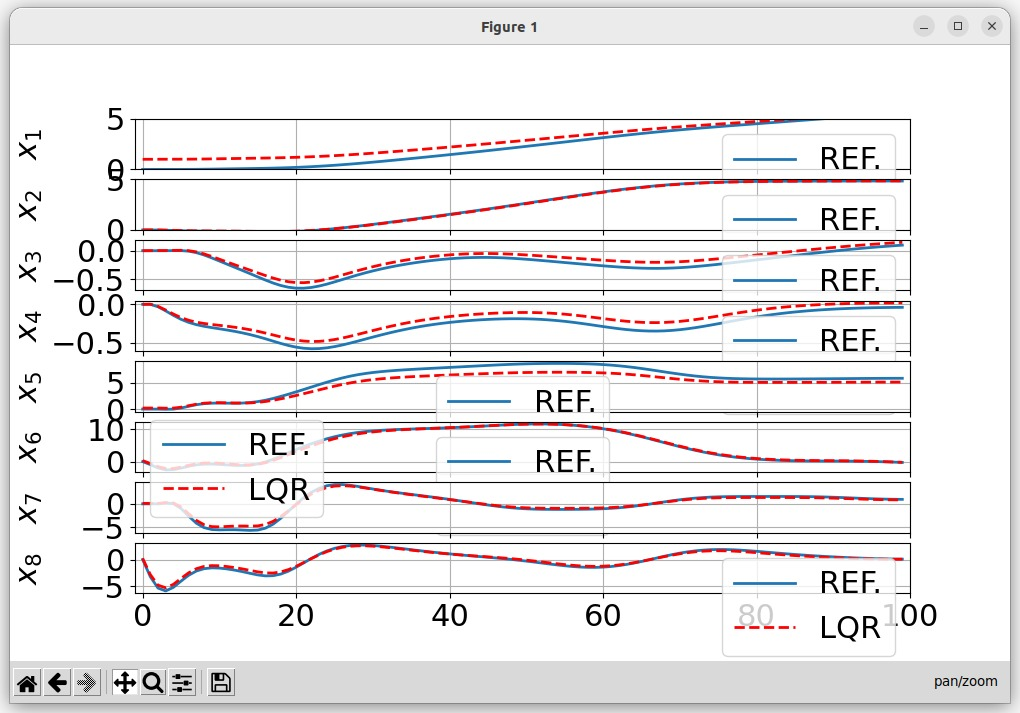
\includegraphics[width=1\textwidth]{figs/Trajectory tracking via LQR 1}
  \end{minipage}
  \caption{State Trajectory Tracking via LQR}
\end{figure}

\begin{figure}[H]
  \begin{minipage}{\linewidth}
  \centering
  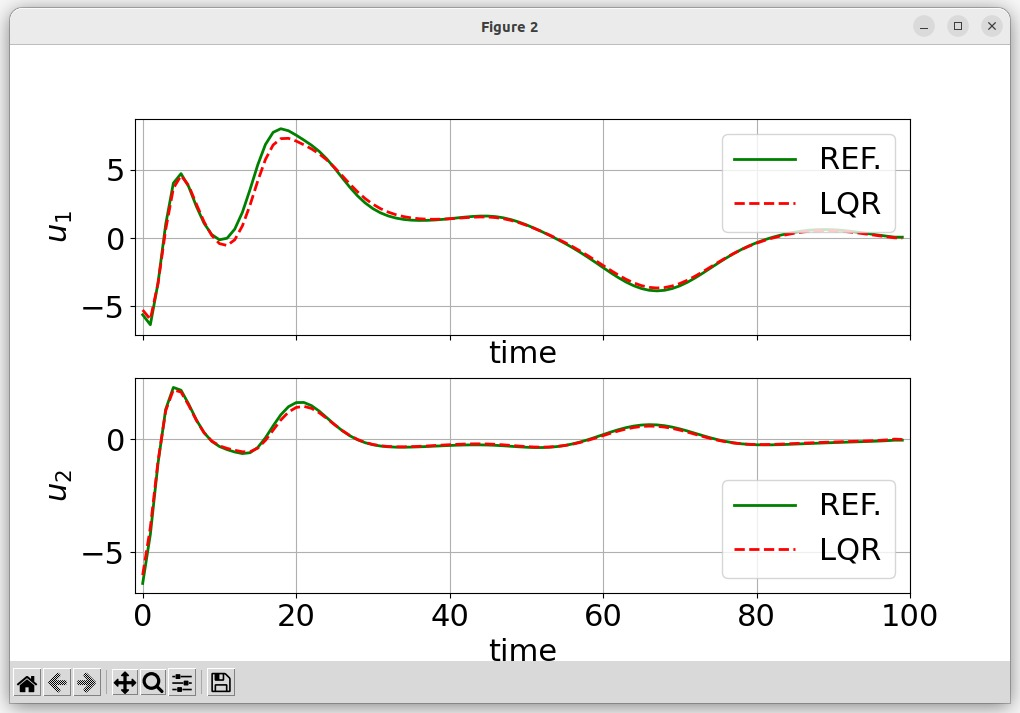
\includegraphics[width=1\textwidth]{figs/Trajectory tracking via LQR 2}
  \end{minipage}
  \caption{Input Trajectory Tracking via LQR}
\end{figure}

\begin{itemize}
     \item From these plots, it is evident that the reference trajectories $x_{1}$ and $x_{2}$ are accurately adhered to. This outcome is positive, considering that these trajectories correspond to the coordinates of the quadrotor's center of mass, reflecting the effective motion of the quadrotor as depicted in the \textbf{animation}.
     \item The remaining variables assume their optimal values based on the provided reference and the dynamics involved (trade-off).
\end{itemize}

\chapter{Task 4 - Trajectory tracking via MPC}
\section{Tracking via MPC}

Idea: For each time instant t, we measure the  current state $x_t$, and then compute the optimal trajectory $x^*_{t\vert t}, ..., x^*_{t+T\vert t}, u^*_{t\vert t}, ..., u^*_{t+T-1\vert t}$ with initial condition $x_t$. After that, we need to apply the first control input $u^*_{t\vert t}$. Finally we measure $x_{t+1}$ and repeat the previous steps to achieve trajectory tracking.\\
\\
\textbf{Solve the optimal control problem at each t}\\

At each time instant t, solve the problem:
\begin{equation*}
\min_{\substack{{x_t,...,x_t+T}\\{u_t,...,u_t+T-1}}} \;  \sum\limits_{\tau=t}^{t+T-1}l_\tau (x_\tau,u_\tau) + l_{t+T} (x_{t+T})\\
\end{equation*}
\begin{equation*}
\textrm{subj. to }x_{\tau+1}=f{(x_\tau,u_\tau)} \quad \forall \tau = t, ..., t+T-1 \\
\end{equation*}
\begin{equation*}
\textrm x_{\tau}\in \chi, u_{\tau}\in \mu \quad \forall \tau = t, ..., t+T \\
\end{equation*}
\begin{equation*}
x_t = x_t^{meas}
\end{equation*}

where
\begin{equation*}
 x_{\tau+1}=f{(x_\tau,u_\tau)}\, is \, the \, so-called \, prediction \, model
\end{equation*}
\begin{equation*}
 x_t^{meas}\, state \, (of \, the \, real \, system) \, measured \, at \, t
\end{equation*}
\\
\textbf{MPC: Linear Quadratic Case}\\

Now for our project we need to consider the case where dynamics is linear and the cost quadratic. At each time t, with initial measured state $x_t^{meas}$, we solve the LQ problem:

\begin{equation*}
\min_{\substack{{x_t,...,x_t+T}\\{u_t,...,u_t+T-1}}} \;  \sum\limits_{t=0}^{t+T-1} x_\tau^\top Q_{\tau}x_\tau + u_\tau^\top R_{\tau}u_\tau + x_{t+T}^\top Q_{T} x_{t+T}\\
\end{equation*}
\begin{equation*}
\textrm{subj. to }x_{\tau+1}=A_\tau x_\tau+B_\tau u_\tau \quad \forall \tau = t, ..., t+T-1 \\
\end{equation*}
\begin{equation*}
\textrm x_{\tau}\in \chi, u_{\tau}\in \mu \quad \forall \tau = t, ..., t+T \\
\end{equation*}
\begin{equation*}
x_t = x_t^{meas}
\end{equation*}

where T is the prediction horizon
\begin{equation*}
x_{\tau} \in \mathbb{R}^{n} \, and \, u_{\tau} \in \mathbb{R}^{m}
\end{equation*}
\begin{equation*}
A_{\tau} \in \mathbb{R}^{n \times n}, B_{\tau} \in \mathbb{R}^{n \times m} \, prediction \, model
\end{equation*}
\begin{equation*}
\chi \, connected \, and \, closed, \mu \, compact
\end{equation*}
\begin{equation*}
Q_{\tau} \in \mathbb{R}^{n \times n} \, and \, Q_{\tau} = Q_{\tau}^\top \geq 0 \, for \, all \, \tau
\end{equation*}
\begin{equation*}
R_{\tau} \in \mathbb{R}^{m \times m} \, and \, R_{\tau} = R_{\tau}^\top > 0 \, for \, all \, \tau
\end{equation*}
\begin{equation*}
Q_{T} \in \mathbb{R}^{n \times n} \, and \, Q_{T} = Q_{T}^\top \geq 0
\end{equation*}
\\
\section{Tracked Trajectories}

The controller monitors the trajectories indicated by the red dotted lines, while the blue lines represent the reference (optimal) trajectories.
\begin{figure}[H]
  \begin{minipage}{\linewidth}
  \centering
  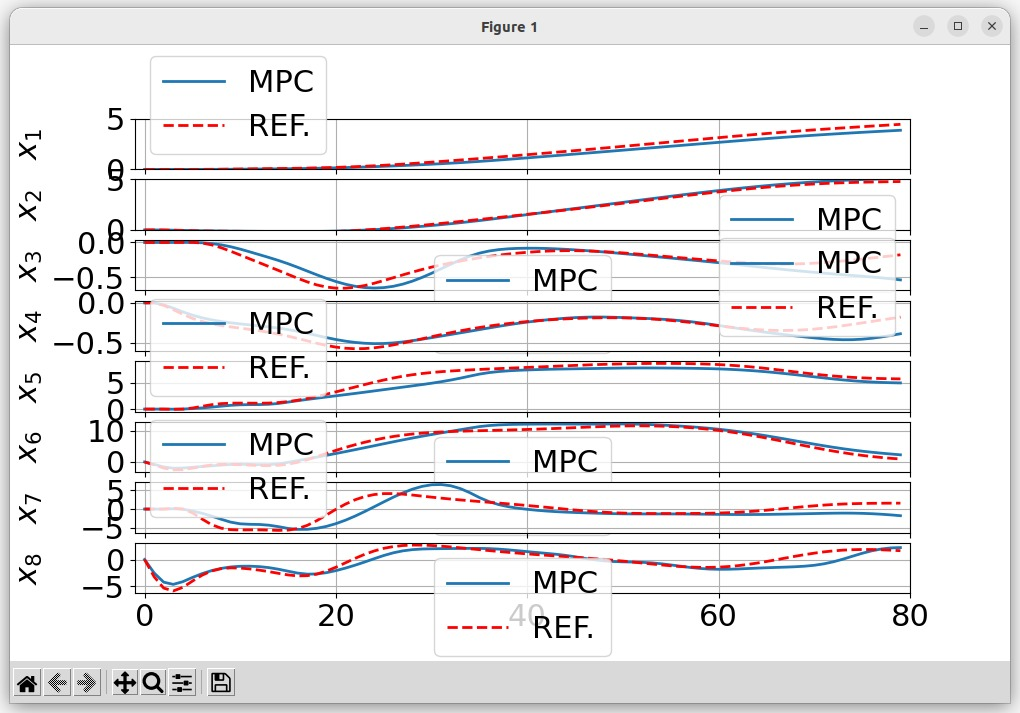
\includegraphics[width=1\textwidth]{figs/Trajectory tracking via MPC 1}
  \end{minipage}
  \caption{State Trajectory Tracking via MPC}
\end{figure}

\begin{figure}[H]
  \begin{minipage}{\linewidth}
  \centering
  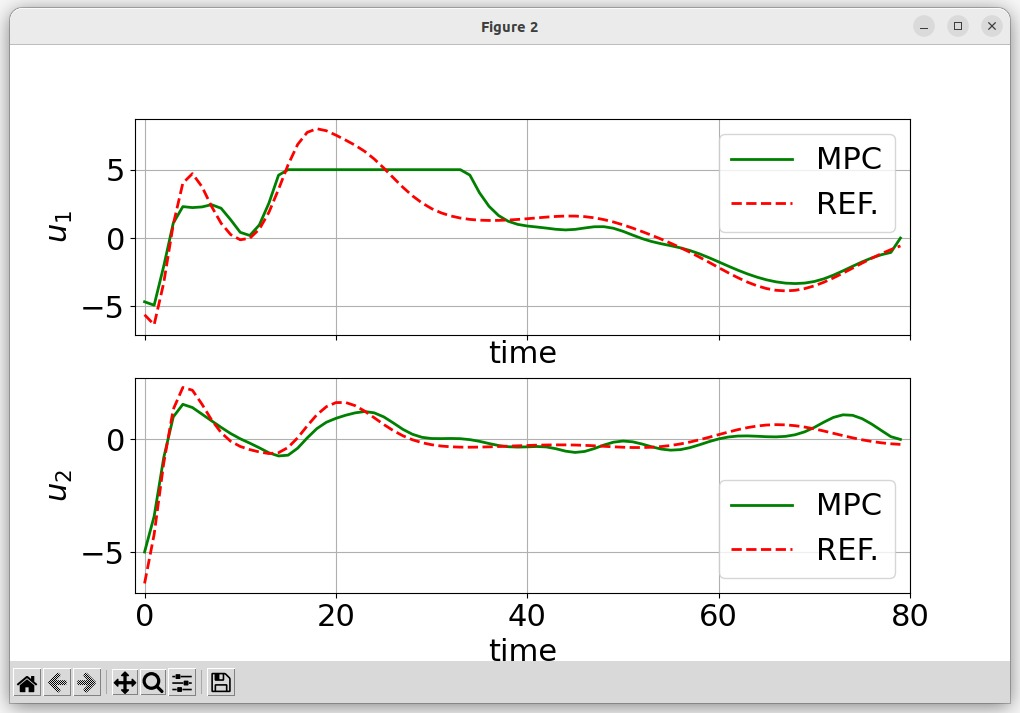
\includegraphics[width=1\textwidth]{figs/Trajectory tracking via MPC 2}
  \end{minipage}
  \caption{Input Trajectory Tracking via MPC}
\end{figure}

\begin{itemize}
     \item The remaining variables assume their optimal values based on the provided reference and the dynamics involved (trade-off).
\end{itemize}

%%%%%%%%%% Conclusions %%%%%%%%%%
\chapter*{Conclusions}
\addcontentsline{toc}{chapter}{Conclusions} 
This project involves employing Newton's Method to generate the optimal trajectory necessary for transitioning from one equilibrium state to another within a discrete non-linear model. The implementation is carried out using Python and comprises three main steps: first, discretizing the dynamic equations; second, establishing a reference trajectory between two flying altitudes; and third, applying Newton's Method to determine the optimal trajectory for the quadrotor to follow. Subsequently, the system is linearized, and feedback controllers as well as MPC algorithms are developed to facilitate tracking of the resulting optimal trajectory.

%%%%%%%%%% Bibliography %%%%%%%%%%%
\bibliography{bibfile}{}
\bibliographystyle{plain}
\addcontentsline{toc}{chapter}{Bibliography}


%%%%%%%%%%%%%%%%%%%%%%%%%%%%%%%%%%%%%%

\end{document}